\documentclass[aps,superscriptaddress,twocolumn,nopreprintnumbers,floatfix,groupedaddress]{revtex4-1}
\usepackage{amssymb}
\usepackage{amsmath}
\usepackage{graphicx}
\usepackage{dcolumn}
\usepackage{hyperref}
\usepackage{color,units}
\usepackage{lineno}
\usepackage{xspace}
\usepackage{mathtools}
\usepackage{physics}
\usepackage{acronym}
\usepackage{subfigure}

\newcommand{\bilby}{{\sc Bilby}\xspace}
\newcommand{\lal}{{\sc LAL}\xspace}
\newcommand{\lalsuite}{{\sc LALSuite}\xspace}
\newcommand{\lalsimulation}{{\sc LALSimulation}\xspace}
\newcommand{\sur}{{\sc NRHybSur3dq8}\xspace}
\newcommand{\Z}{\mathcal{Z}}
\newcommand{\M}{\mathcal{M}}
\renewcommand{\L}{\mathcal{L}}
\newcommand{\BF}{\mathcal{BF}}
\newcommand{\proposal}{proposal}
\newcommand{\target}{target}
\newcommand{\ep}[1]{\textcolor{red}{[EP: #1]}}
\newcommand{\et}[1]{\textcolor{blue}{[ET: #1]}}
\newcommand{\ct}[1]{\textcolor{green}{[CT: #1]}}

\newcommand{\nessai}{{\sc Nessai}\xspace}
\newcommand{\vitamin}{{\sc VItamin}\xspace}
\newcommand{\bilbypipe}{{\sc bilby\_pipe}\xspace}
\newcommand{\lalinference}{{\sc LALInference}\xspace}
\newcommand{\dynesty}{{\sc dynesty}\xspace}
\newcommand{\cpnest}{{\sc cpnest}\xspace}
\newcommand{\nflows}{{\sc nflows}\xspace}
\newcommand{\pytorch}{{\sc PyTorch}\xspace}
\newcommand{\corner}{{\sc corner}\xspace}
\newcommand{\matplotlib}{{\sc matplotlib}\xspace}
\newcommand{\seaborn}{{\sc seaborn}\xspace}
\newcommand{\numpy}{{\sc NumPy}\xspace}
\newcommand{\scipy}{{\sc SciPy}\xspace}
\newcommand{\pandas}{{\sc pandas}\xspace}
\newcommand{\python}{{\sc Python}\xspace}
\newcommand{\imrphenomp}{{\sc IMRPhenomPv2}\xspace}


\newcommand{\figwidth}{8.6cm}
\newcommand{\onehalffigwidth}{12.9cm}
\newcommand{\doublefigwidth}{17.2cm}
\newcommand{\montefigwidth}{11cm}

\begin{document}

\title{Explainable Deep-learning: Monte Carlo methods for Gravitational-Wave Inference}

\author{Project No:~628}
%\email{ethan.payne@ligo.org}
\affiliation{%
	SUPA, School of Physics and Astronomy \\
	University of Glasgow \\
	Glasgow G12 8QQ, United Kingdom
}%

\date{\today}

\begin{abstract}
My 250 word abstract goes here...
\end{abstract}

\maketitle

\acrodef{GW}[GW]{Gravitational wave}
\acrodef{BBH}[BBH]{binary black hole}
\acrodef{EM}[EM]{electromagnetic}
\acrodef{CBC}[CBC]{compact binary coalescence}
\acrodef{BNS}[BNS]{binary neutron star}
\acrodef{NSBH}[NSBH]{neutron star black hole}
\acrodef{PSD}[PSD]{power spectral density}
\acrodef{ELBO}[ELBO]{evidence lower bound}
\acrodef{LIGO}[LIGO]{advanced Laser Interferometer Gravitational wave Observatory}
\acrodef{CVAE}[CVAE]{conditional variational autoencoder}
\acrodef{KL}[KL]{Kullback--Leibler}
\acrodef{GPU}[GPU]{graphics processing unit}
\acrodef{LVC}[LVC]{LIGO-Virgo Collaboration}
\acrodef{PP}[p-p]{probability-probability}
\acrodef{SNR}[SNR]{signal-to-noise ratio}

\section{Introduction}\label{intro}

\textbf{\textcolor{red}{Figs: Hunter's Vit Schematic}}

\textbf{\textcolor{green}{Tables: Compare inference speeds like in vit paper}}

Remember to signpost rest of paper at end of this section!

%\subsection{}
%
\subsection{\vitamin: User-Friendly Inference}\label{vit}

\textbf{\textcolor{green}{Tables: Compare Gen Model abilities}}

Use gen pap to intro CVAE in context, CONTEXT IS KEY HERE


\begin{figure}
	\centering
	
\includegraphics[width=\figwidth]{figs/network_setup.png}
	\caption{Example of how a normalising flow trained on a set of live points can produce samples within current iso-likelihood contour for simple two-dimensional parameter space. \textbf{Top:} example of training samples in the physical space $\physical$ and learned mapping to the latent space $\latent$ with the iso-likelihood contour for the current \textit{worst point} shown in orange. \textbf{Middle:} samples drawn from a truncated Guassian within the iso-likelihood contour in $\latent$ and mapped to $\physical$ using the inverse mapping. \textbf{Bottom:} pool of accepted samples after applying rejection sampling until 1000 points are obtained shown in both $\latent$ and $\physical$.}
	\label{fig:vit_flow}
\end{figure}

%
%\subsection{Structure}
%
%\subsection{Training}
%
%\subsection{Results}

%\section{Theoretical Framework}\label{theory}

Need to mention metropolis hastings it seems!

Introduce equations directly to our specifics, we don't have space to intro them blind then again to specifics...

\subsection{Monte Carlo Framework}\label{theory:monte}

\subsection{SIR Framework}\label{theory:sir}

Do theory on normal IS and then say that SIR is an monte carlo approach/approx to normal IS then give equations for bot (talk about the NEW IMPROVED SIR method (link to Section \ref{future}))

%
%\subsection{Theoretical Framework}\label{monte:theory}

\section{Methodology}\label{methods}

Apply the intro/theory mateiral to our case, JUSTIFY scientific decisions like number of samples, batch size, npars!!

\subsection{Model Training}

\begin{figure}
	\centering
	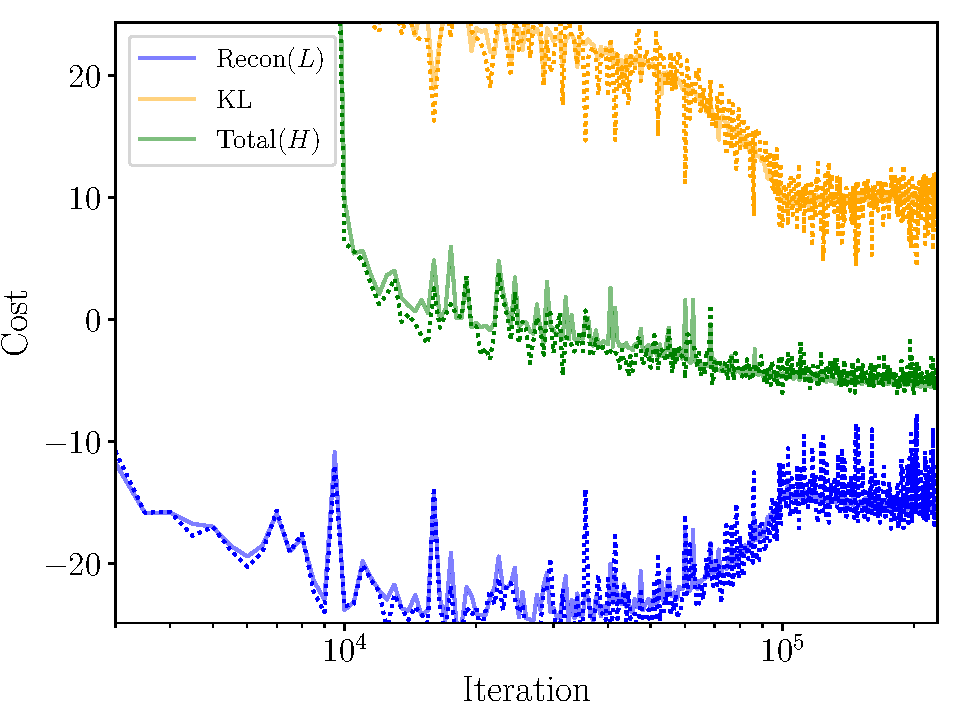
\includegraphics[width=\figwidth]{figs/cost.pdf}
	\caption{Example of how a normalising flow trained on a set of live points can produce samples within current iso-likelihood contour for simple two-dimensional parameter space. \textbf{Top:} example of training samples in the physical space $\physical$ and learned mapping to the latent space $\latent$ with the iso-likelihood contour for the current \textit{worst point} shown in orange. \textbf{Middle:} samples drawn from a truncated Guassian within the iso-likelihood contour in $\latent$ and mapped to $\physical$ using the inverse mapping. \textbf{Bottom:} pool of accepted samples after applying rejection sampling until 1000 points are obtained shown in both $\latent$ and $\physical$.}
	\label{fig:learning_contours}
\end{figure}

\begin{figure*}
	\subfigure{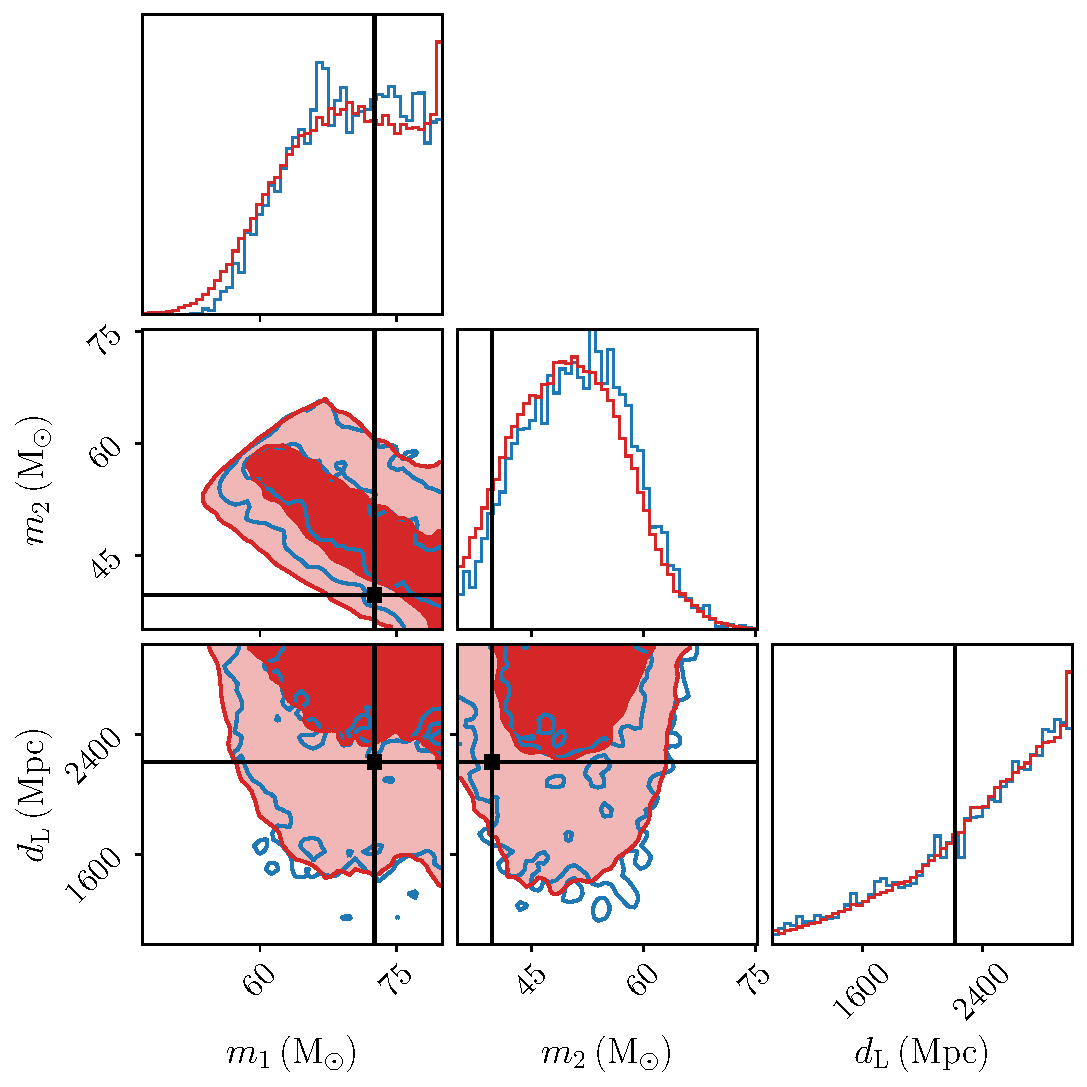
\includegraphics[width=\figwidth]{figs/vit_train_corner1.pdf}}
	\subfigure{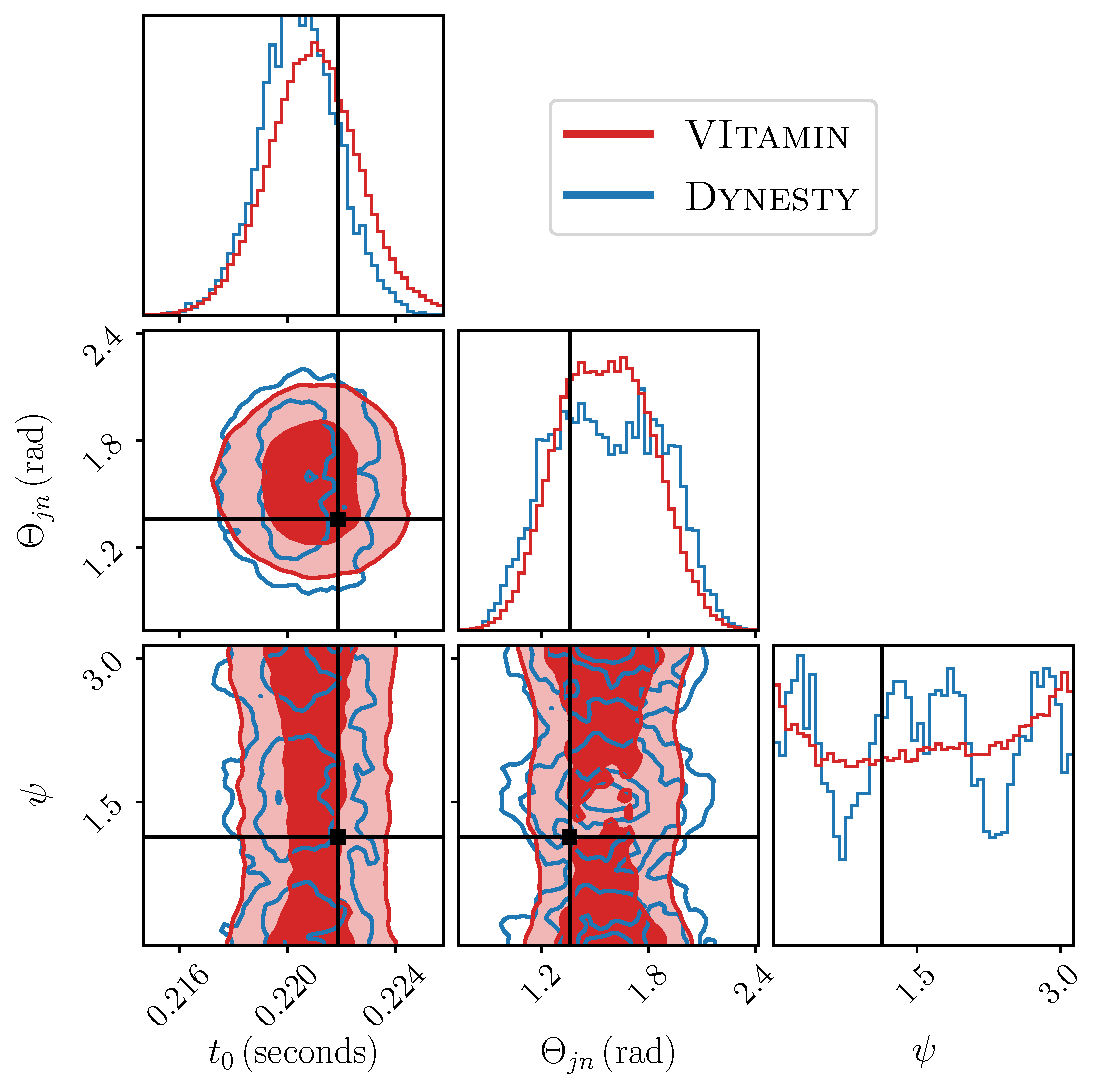
\includegraphics[width=\figwidth]{figs/vit_train_corner2.pdf}}
	\caption{Probability-probability (P-P) plot showing the confidence interval versus the fraction of the events within that confidence interval for the posterior distributions obtained using our analysis \nessai for 128 simulated compact binary coalescence signals produced with \bilby and \bilbypipe. The 1-, 2- and 3-$\sigma$ confidence intervals are indicated by the shaded regions and $p$-values are shown for each of the parameters and the combined $p$-value is also shown.}
	\label{fig:vit_train_corner}
\end{figure*}

\textbf{\textcolor{red}{Figs: loss plot}}

\textbf{\textcolor{green}{Tables: training hypers in table}}

\textbf{\textcolor{red}{Figs: initial corner plot? (to talk about params and how posteriors aren't perfect)}}

Need this cornerplot here to talk about how it doesn't `get' the multimodal dists, which after resampling it does!

\subsection{Likelihood Estimates}

\textbf{\textcolor{red}{Figs: Monte flowchart}}

\begin{figure*}
	\centering
	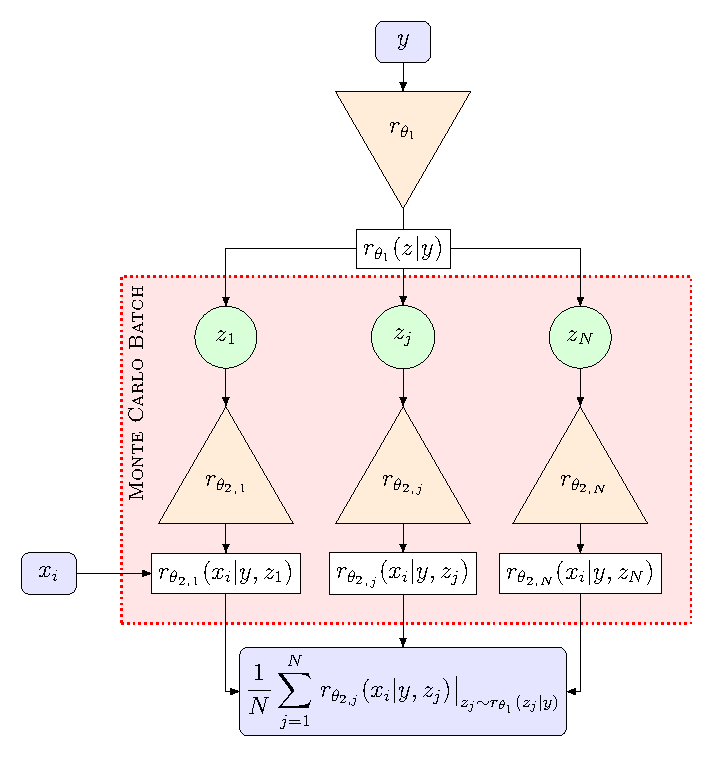
\includegraphics[width=\montefigwidth]{figs/tikz_monte.pdf}
	\caption{Diagram of a normalising flow $f(x)$ composed of four coupling transforms which maps an \protect\ndimensional{n} input vector x to an \protect\ndimensional{n} latent vector z. Each transform splits $x$ in two $[x_{1:m}, x_{m+1:n}]$ and updates one part conditioned on the other. In the first and third transforms $x_{1:m}$ is used as the input to a neural network (NN) which then produces the scale $s$ and translation $t$ vectors of length $m$. The element-wise product ($\odot$) is then computed between $x_{1:m}$ and $\exp(s)$ followed by the sum of the output and $t$. This is shown in the left transform. In the second and fourth transforms $x_{1:m}$ is updated conditioned on $x_{m+1:n}$ as shown in the right transform. \textcolor{red} {In my caption, link to previous sections and equations}}
	\label{fig:monte_flow}
\end{figure*}


\subsection{Importance Resampling}


\section{Results}\label{results}

\subsection{Self-consistency}

\textbf{\textcolor{red}{Figs: Self consist corner plot}}

\begin{figure*}
	\subfigure{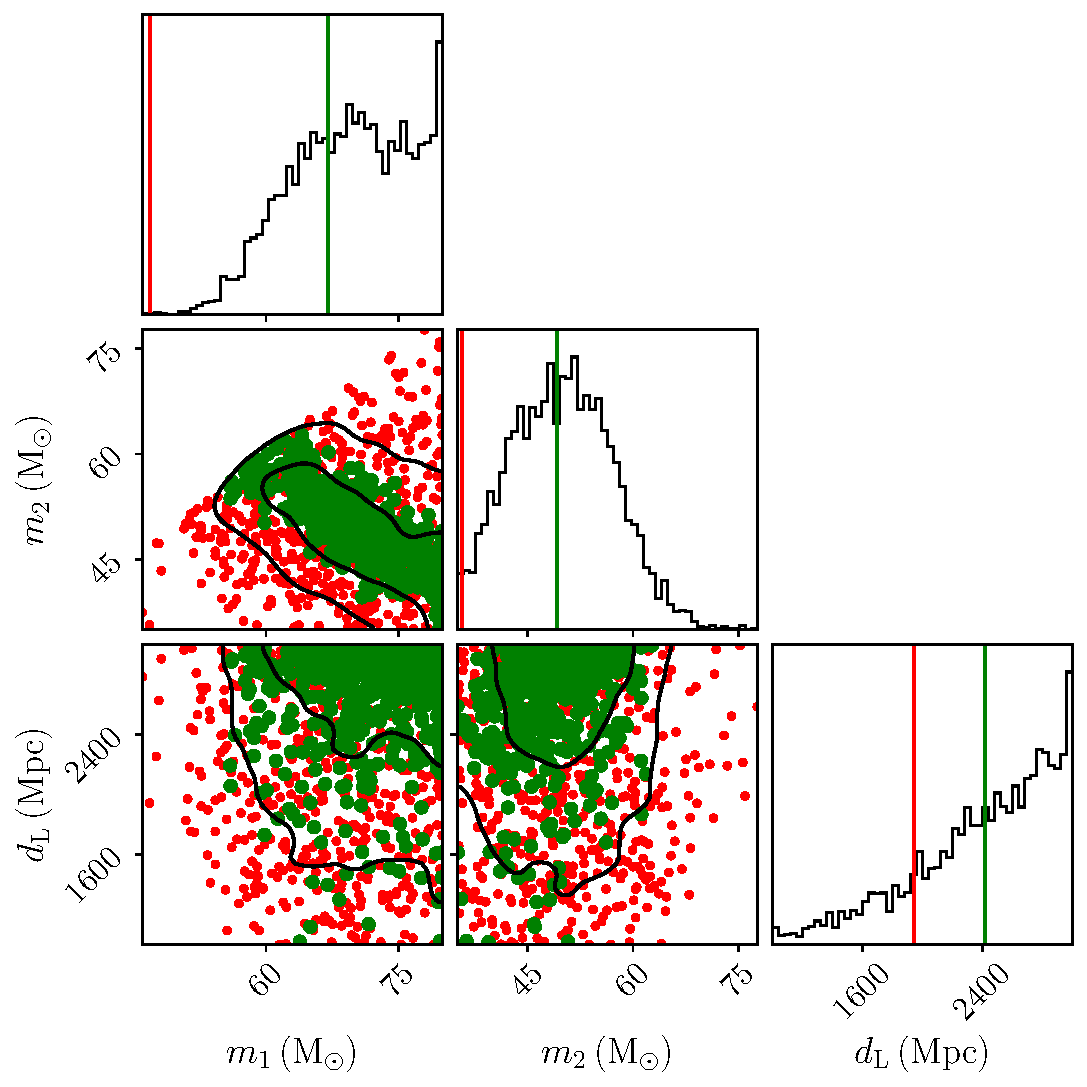
\includegraphics[width=\figwidth]{figs/self_consist1.pdf}}
	\subfigure{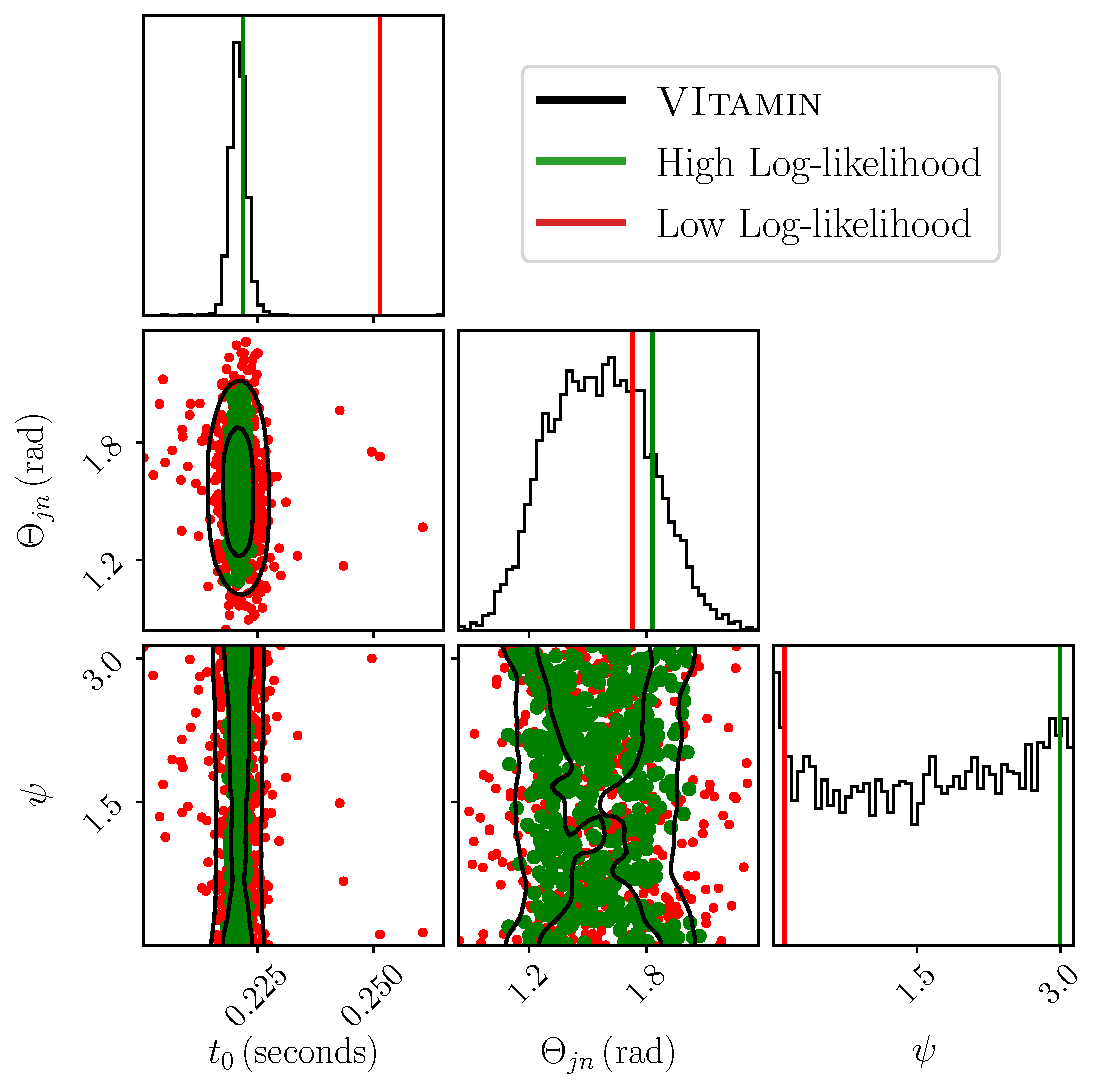
\includegraphics[width=\figwidth]{figs/self_consist2.pdf}}
	\caption{Probability-probability (P-P) plot showing the confidence interval versus the fraction of the events within that confidence interval for the posterior distributions obtained using our analysis \nessai for 128 simulated compact binary coalescence signals produced with \bilby and \bilbypipe. The 1-, 2- and 3-$\sigma$ confidence intervals are indicated by the shaded regions and $p$-values are shown for each of the parameters and the combined $p$-value is also shown.}
	\label{fig:sel_consist}
\end{figure*}


\subsection{Reproducibility}

Talk about how 'binning' is preventing proper error profile acorss the likelihood range, (not present in the \dynesty case)

\textbf{\textcolor{red}{Figs: sigma gaussians for different z batch}}

\begin{figure}
	\centering
	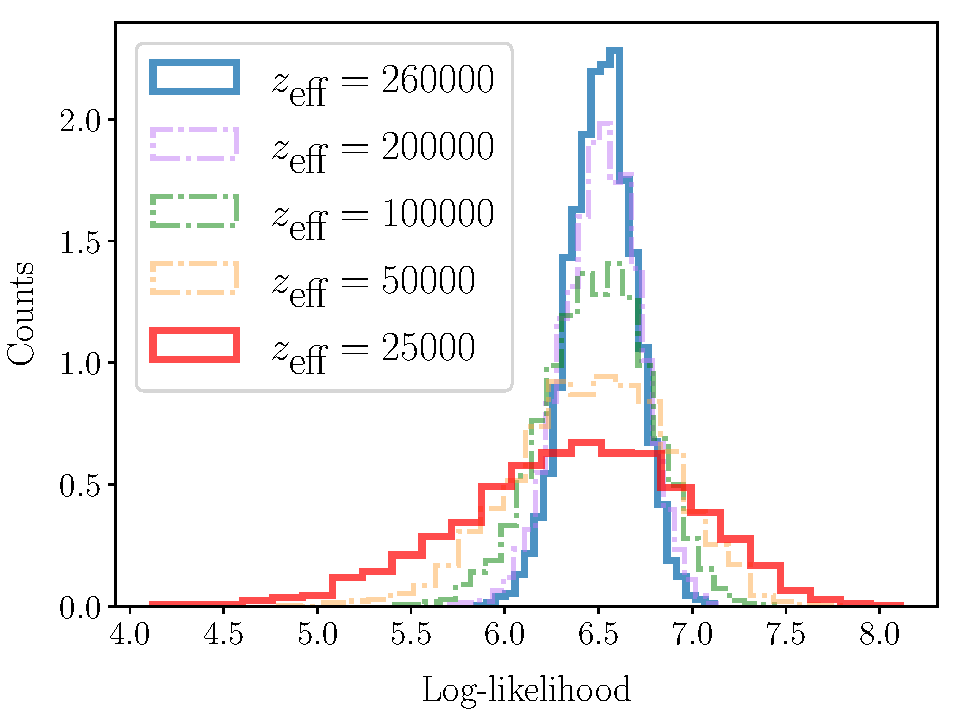
\includegraphics[width=\figwidth]{figs/hists_rect.pdf}
	\caption{Example of how a normalising flow trained on a set of live points can produce samples within current iso-likelihood contour for simple two-dimensional parameter space. \textbf{Top:} example of training samples in the physical space $\physical$ and learned mapping to the latent space $\latent$ with the iso-likelihood contour for the current \textit{worst point} shown in orange. \textbf{Middle:} samples drawn from a truncated Guassian within the iso-likelihood contour in $\latent$ and mapped to $\physical$ using the inverse mapping. \textbf{Bottom:} pool of accepted samples after applying rejection sampling until 1000 points are obtained shown in both $\latent$ and $\physical$.}
	\label{fig:hists}
\end{figure}



\textbf{\textcolor{red}{Figs: scatter vit vit}}

\textbf{\textcolor{red}{Figs: scatter vit dynesty}}


\begin{figure*}
	\subfigure[]{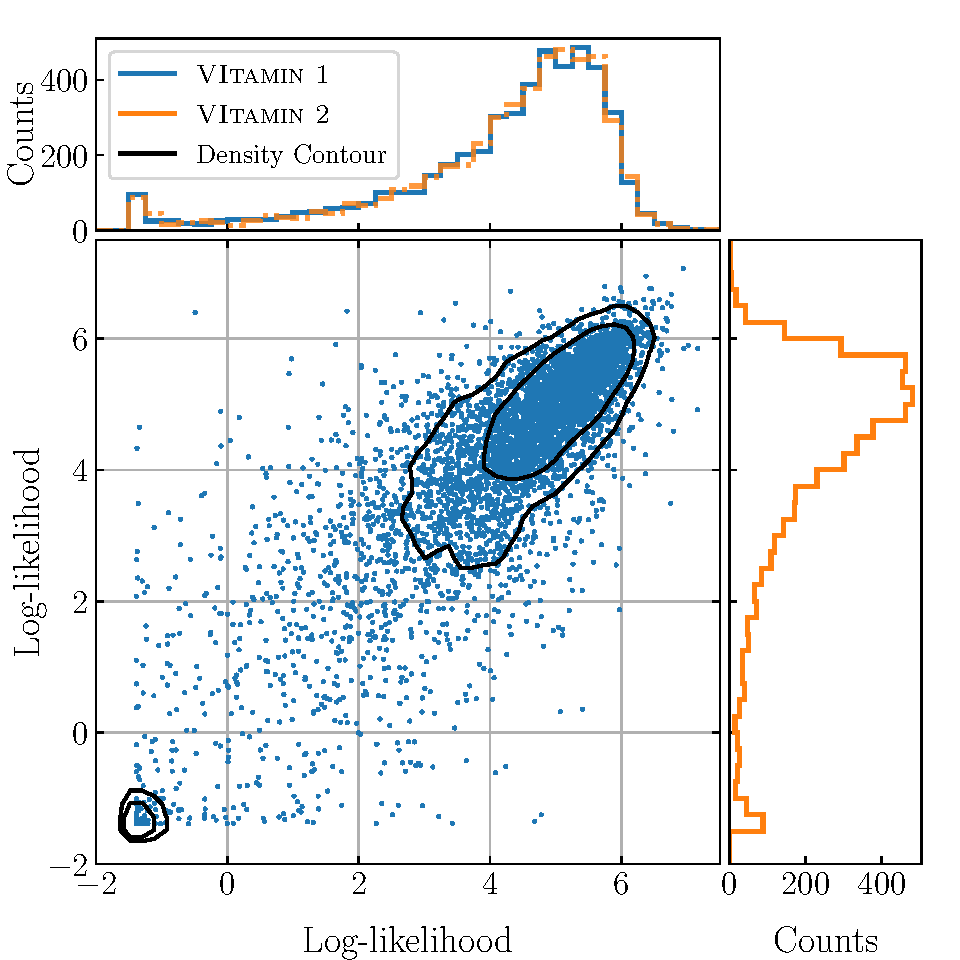
\includegraphics[width=\figwidth]{figs/vvscatter.pdf}}
	\subfigure[]{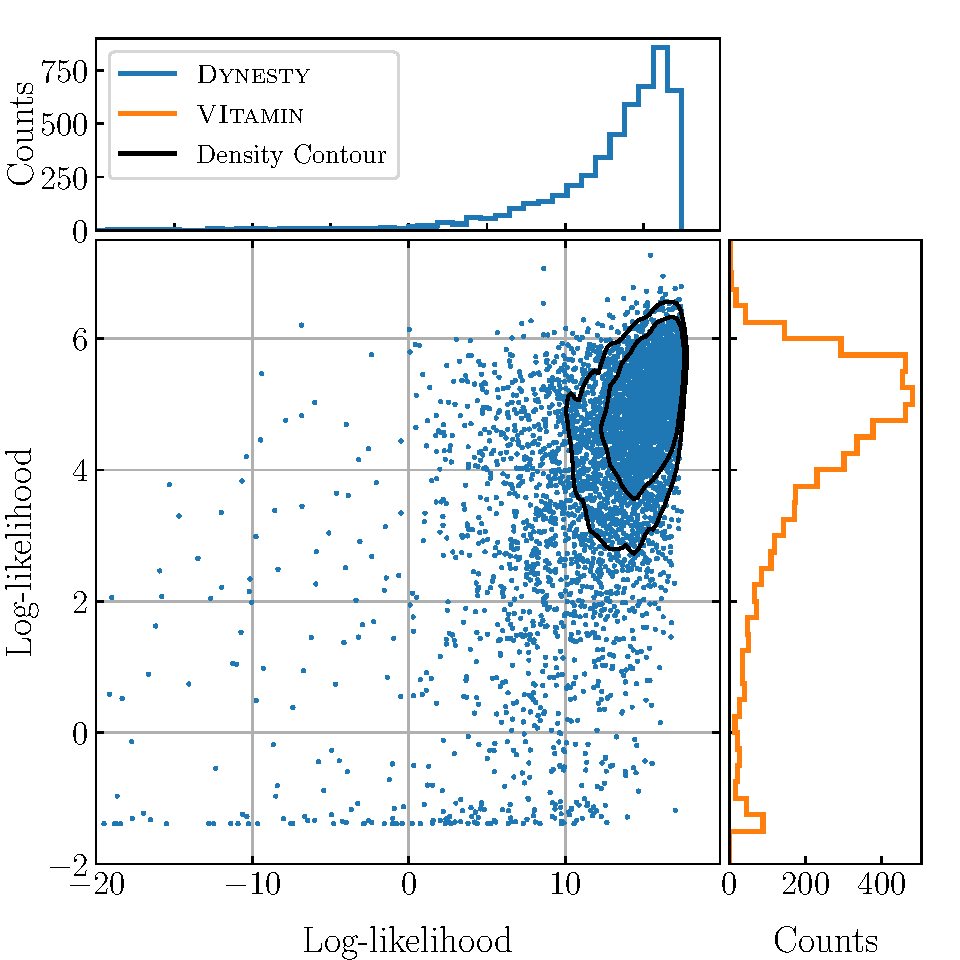
\includegraphics[width=\figwidth]{figs/bvscatter.pdf}}
	\caption{Probability-probability (P-P) plot showing the confidence interval versus the fraction of the events within that confidence interval for the posterior distributions obtained using our analysis \nessai for 128 simulated compact binary coalescence signals produced with \bilby and \bilbypipe. The 1-, 2- and 3-$\sigma$ confidence intervals are indicated by the shaded regions and $p$-values are shown for each of the parameters and the combined $p$-value is also shown.}
	\label{fig:scatter}
\end{figure*}

\subsection{Importance Resampling}


\textbf{\textcolor{red}{Figs: Final corner plot (big)}}

\begin{figure*}[h]
	\centering
	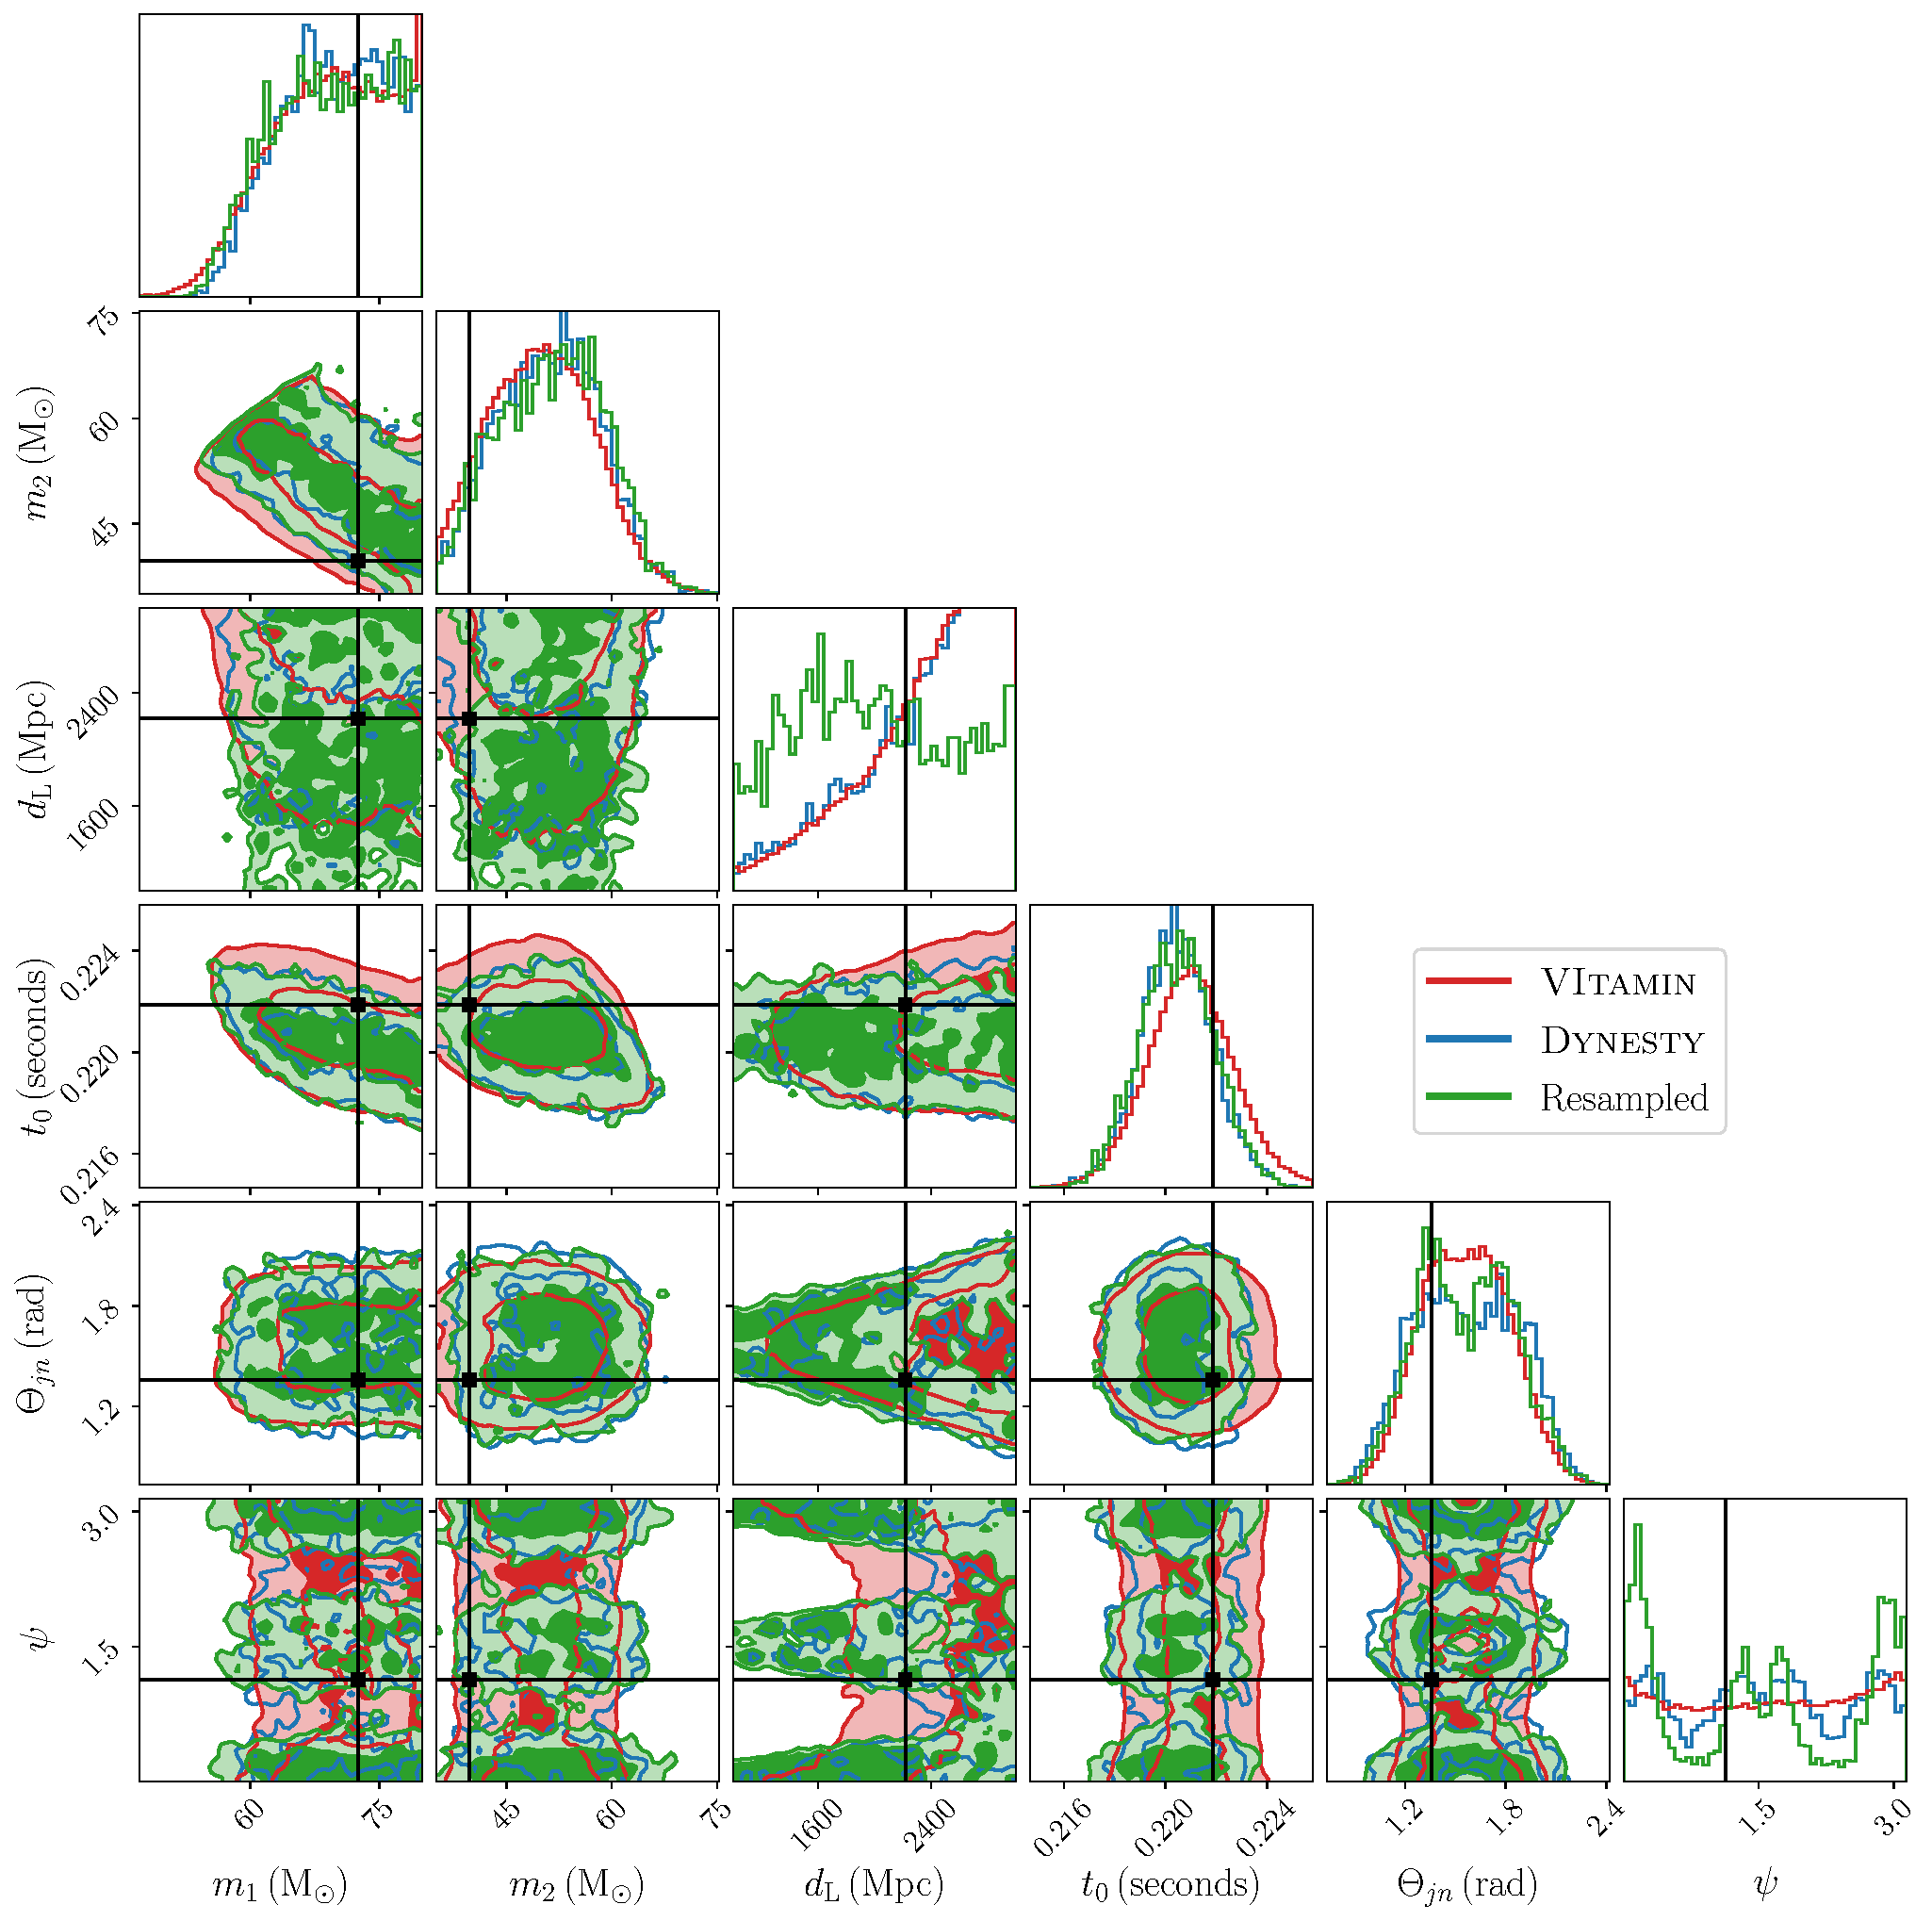
\includegraphics[width=\doublefigwidth]{figs/resample_corner.pdf}
	\caption{Corner plot comparing the posterior distributions produced with \dynesty (blue) and our sampler \nessai (red). The phase is marginalised and remaining 14 parameters are shown, see \cref{app:priors} for details on the parameters. The respective 16\% and 84\% quantiles are also shown in the \protect\ndimensional{1} marginalised posteriors.}
	\label{fig:final_corner}
\end{figure*}

%\section{Future Work}\label{future}


\section{Conclusions}\label{conc}

This is section has to encapsulate everything we did so that after the abstract a reader can go here and see if they want to buy the paper or not!

As we find ourself in a proof-of-concept mode, there is justification of a section dedicated to the next steps leading towards production of this code.


\section*{Acknowledgements}

Thanks to Chris and Hunter and Michael and Daniel.

Paragraph on the software used \bilby\cite{bilby} 
%\clearpage
\bibliography{refs}




\end{document}